\section{Gradient Computation}
I managed to successfully write the functions to correctly compute the gradient analytically.
I tested my implementation by computing the gradients using both ComputeGradsNum.m and ComputeGradsNumSlow.m.
Then I compared my results with the numerical approaches by calculating the absolute difference of each gradient element as in equation
\eqref{eq:diffw} and \eqref{eq:diffb}. 
Then I checked those against a threshold (1e-6). I also used the other formula that was given in the assignment instructions to
compare the error (equation \eqref{eq:diffw2} and \eqref{eq:diffb2}).
Depending on the seed sometimes I got an error that was larger than 1e-6 (e.g. 3e-6) but this error is still
small enough to conclude that my implementation works.\\

\begin{equation}\label{eq:diffw}
    diff\_W = abs(ngrad\_W - grad\_W)
\end{equation}
\begin{equation}\label{eq:diffb}
    diff\_b = abs(ngrad\_b - grad\_b)
\end{equation}

\begin{equation}\label{eq:diffw2}
    diff\_W = abs(ngrad\_W - grad\_W)./max(eps, abs(grad\_W) + abs(ngrad\_W))
\end{equation}
\begin{equation}\label{eq:diffb2}
    diff\_b = abs(ngrad\_b - grad\_b)./max(eps, abs(grad\_b) + abs(ngrad\_b))
\end{equation}

\section{Results} 
\label{sec:results}

\begin{table}[ht]
\begin{tabular}{|l|l|l|l|l|}
\hline
                   & \textbf{Experiment 1} & \textbf{Experiment 2} & \textbf{Experiment 3} & \textbf{Experiment 4} \\ \hline
\textbf{seed}      & 400                   & 400                   & 400                   & 400                   \\ \hline
\textbf{lambda}    & 0                     & 0                     & 0.1                   & 1                     \\ \hline
\textbf{n\_batch}  & 100                   & 100                   & 100                   & 100                   \\ \hline
\textbf{eta}       & 0.1                   & 0.001                 & 0.001                 & 0.001                 \\ \hline
\textbf{n\_epochs} & 40                    & 40                    & 40                    & 40                    \\ \hline
\end{tabular}
\caption{Experiment parameters}
\label{tab:experiment_parameters}
\end{table}

\begin{table}[ht]
\begin{tabular}{|l|l|l|l|l|}
\hline
                    & \textbf{Experiment 1} & \textbf{Experiment 2} & \textbf{Experiment 3} & \textbf{Experiment 4} \\ \hline
\textbf{Training}   & 5.074                 & 1.609                 & 0.3908                & 1.899                 \\ \hline
\textbf{Validation} & 7.526                 & 1.791                 & 1.903                 & 1.958                 \\ \hline
\end{tabular}
\caption{Summary of final loss}
\label{tab:summary_loss}
\end{table}

\begin{table}[ht]
\begin{tabular}{|l|l|l|l|l|}
\hline
                  & \textbf{Experiment 1} & \textbf{Experiment 2} & \textbf{Experiment 3} & \textbf{Experiment 4} \\ \hline
\textbf{Accuracy} & 27.84\%               & 39.08\%               & 39.46\%               & 37.38\%               \\ \hline
\end{tabular}
\caption{Summary of final accuracy}
\label{tab:summary_accuracy}
\end{table}

\newpage

\subsection{Experiment 1 diagrams}
% lambda = 0\\
% n\_epochs = 40\\
% n\_batch = 100\\
% eta = 0.1\\
As seen in the diagrams with the parameters of this run the network is not really able to learn. The loss and accuracy look very random. 
This results in a very low accuracy (27.84\%). The weight matrices look pretty random as well.

    \begin{figure}[ht]
        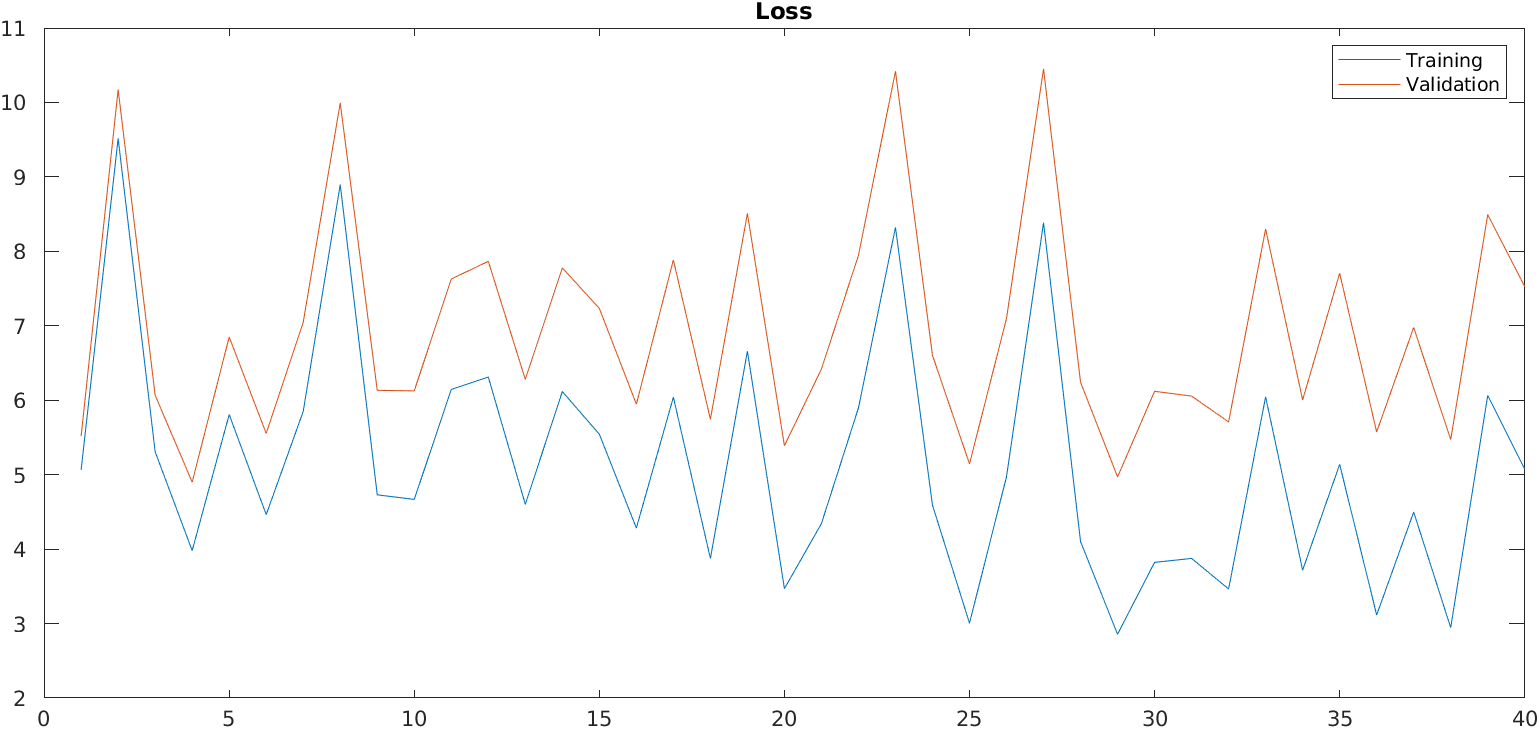
\includegraphics[width=\textwidth]{../code/result_pics/lambda=0, n_epochs=40, n_batch=100, eta=.1/loss.png}
        \caption{Experiment 1 Loss (lambda=0, n\_epochs=40, n\_batch=100, eta=0.1)}
        \label{fig:loss1}
    \end{figure}

    \begin{figure}[ht]
        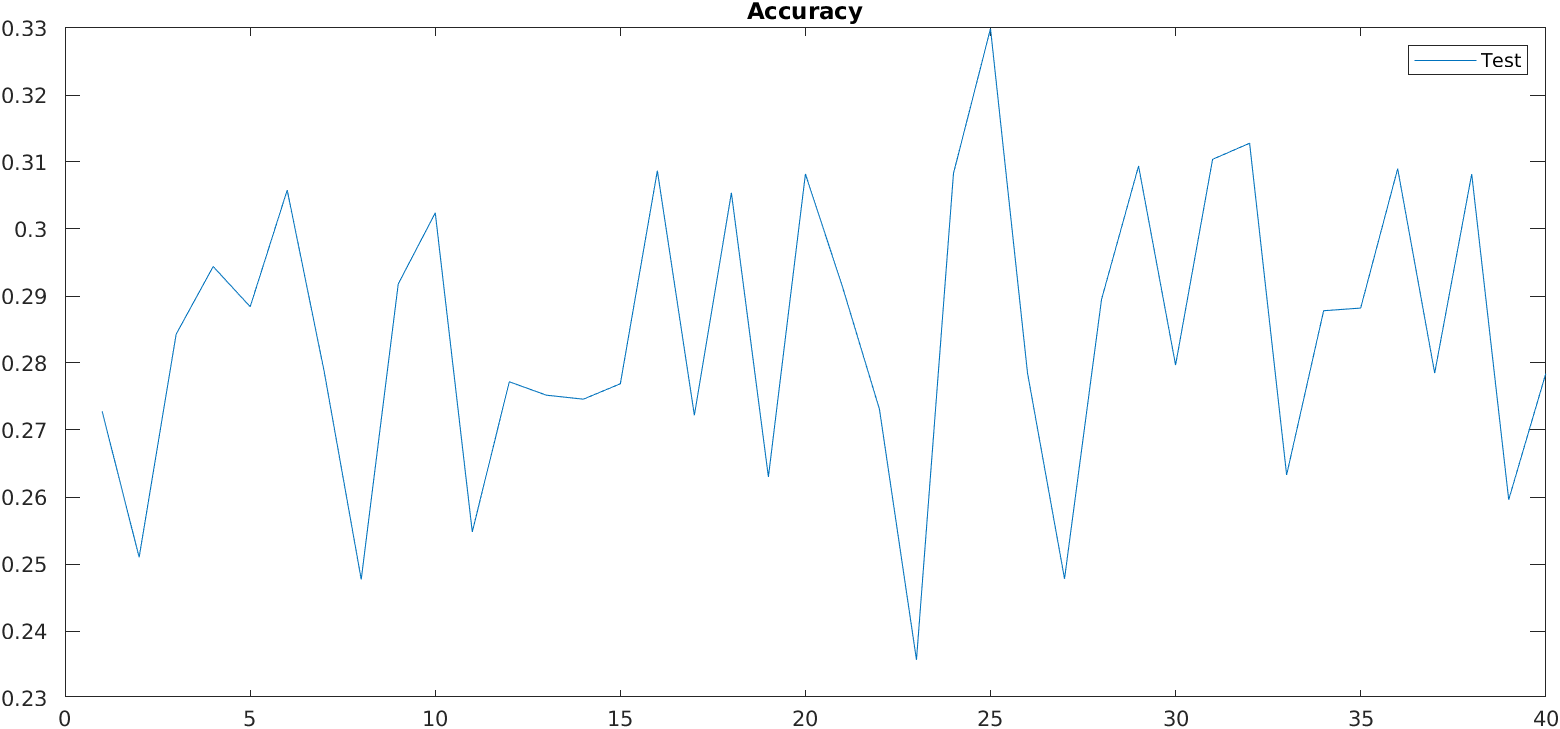
\includegraphics[width=\textwidth]{../code/result_pics/lambda=0, n_epochs=40, n_batch=100, eta=.1/accuracy.png}
        \caption{Experiment 1 Accuracy (lambda=0, n\_epochs=40, n\_batch=100, eta=0.1)}
        \label{fig:accuracy1}
    \end{figure}

    \begin{figure}[ht]
        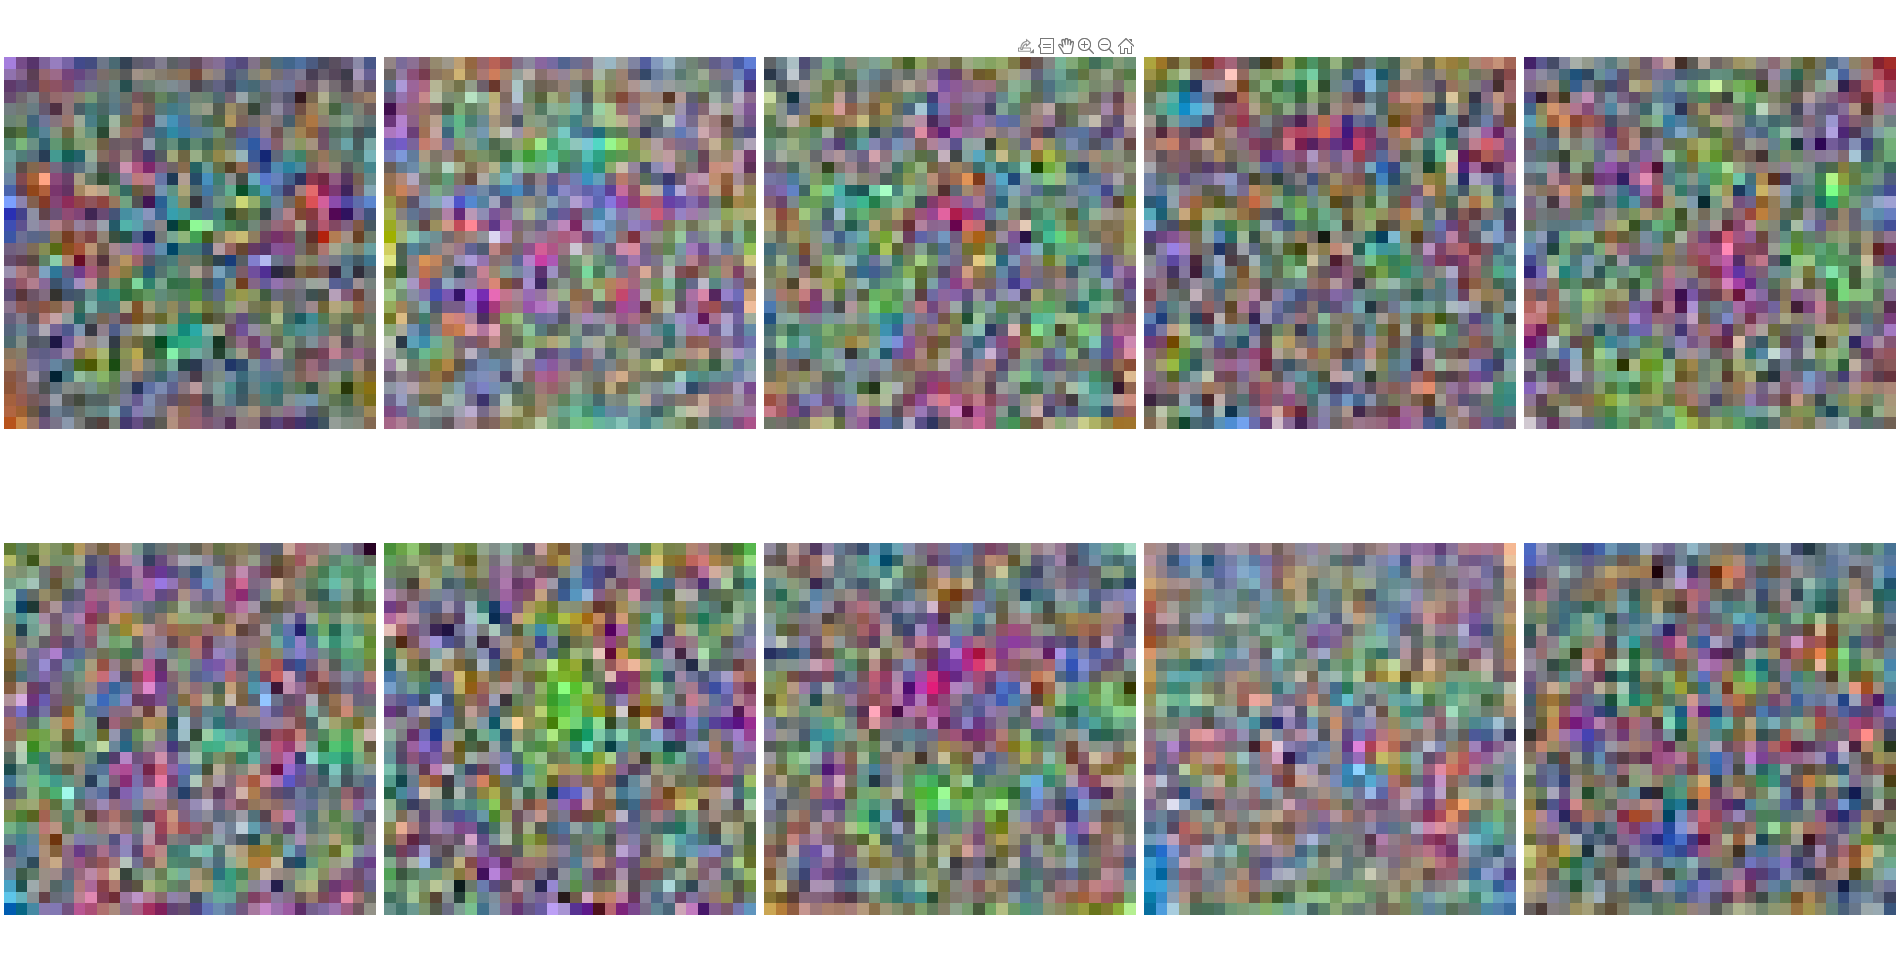
\includegraphics[width=\textwidth]{../code/result_pics/lambda=0, n_epochs=40, n_batch=100, eta=.1/weights.png}
        \caption{Experiment 1 Weights (lambda=0, n\_epochs=40, n\_batch=100, eta=0.1)}
        \label{fig:weights1}
    \end{figure}

\clearpage
\subsection{Experiment 2 diagrams}
% lambda = 0\\
% n\_epochs = 40\\
% n\_batch = 100\\
% eta = 0.1\\
Compared to the first experiment in this run we use a much smaller learning rate. In this run it looks like the network learns better and it results in a higher
accuracy (39.08\%). If we look at the loss graphs we can see that there is a big difference between the training loss and validation loss. 
This could be an indicator for overfitting. The weight matrices look less random.

    \begin{figure}[ht]
        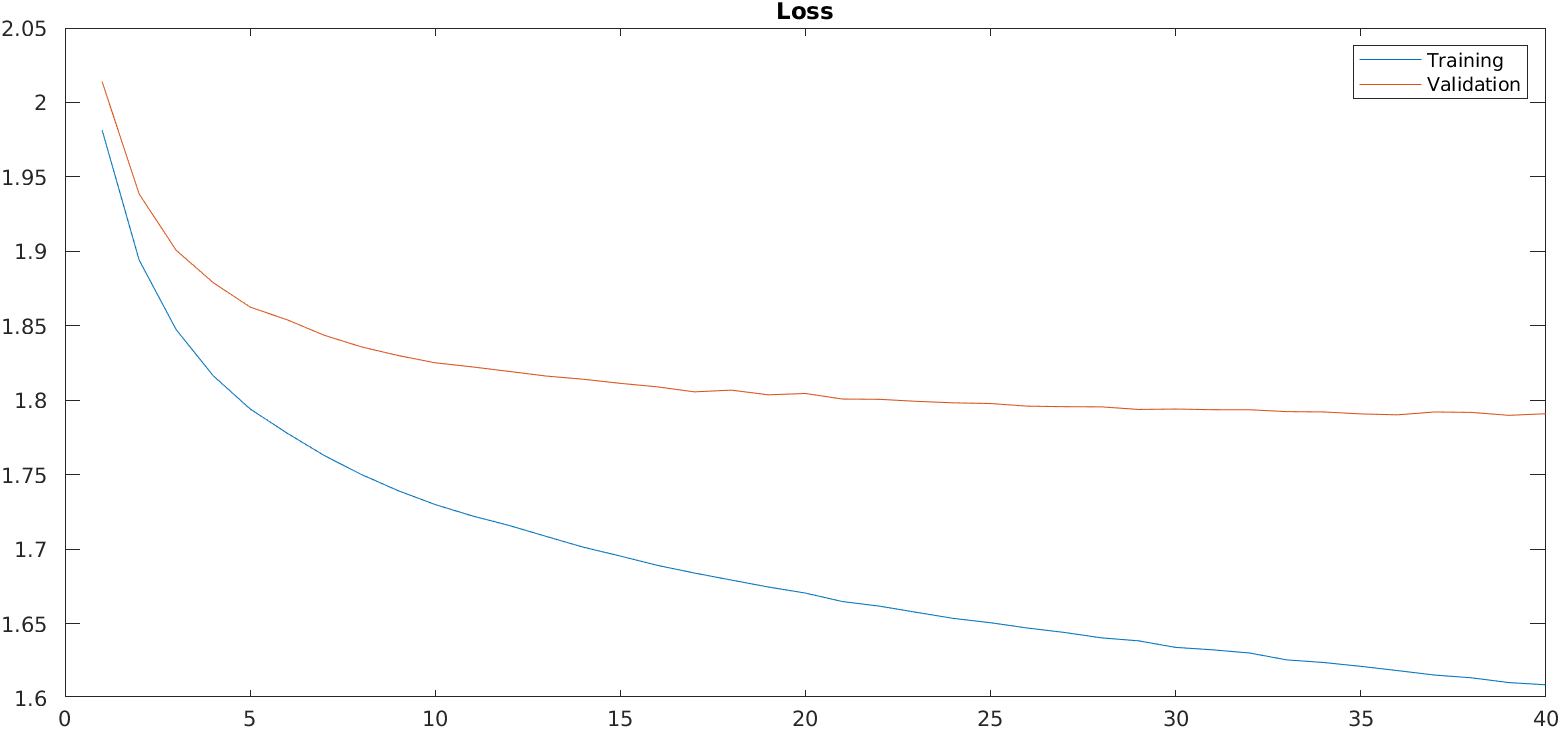
\includegraphics[width=\textwidth]{../code/result_pics/lambda=0, n_epochs=40, n_batch=100, eta=.001/loss.png}
        \caption{Experiment 2 Loss (lambda=0, n\_epochs=40, n\_batch=100, eta=0.001)}
        \label{fig:loss2}
    \end{figure}

    \begin{figure}[ht]
        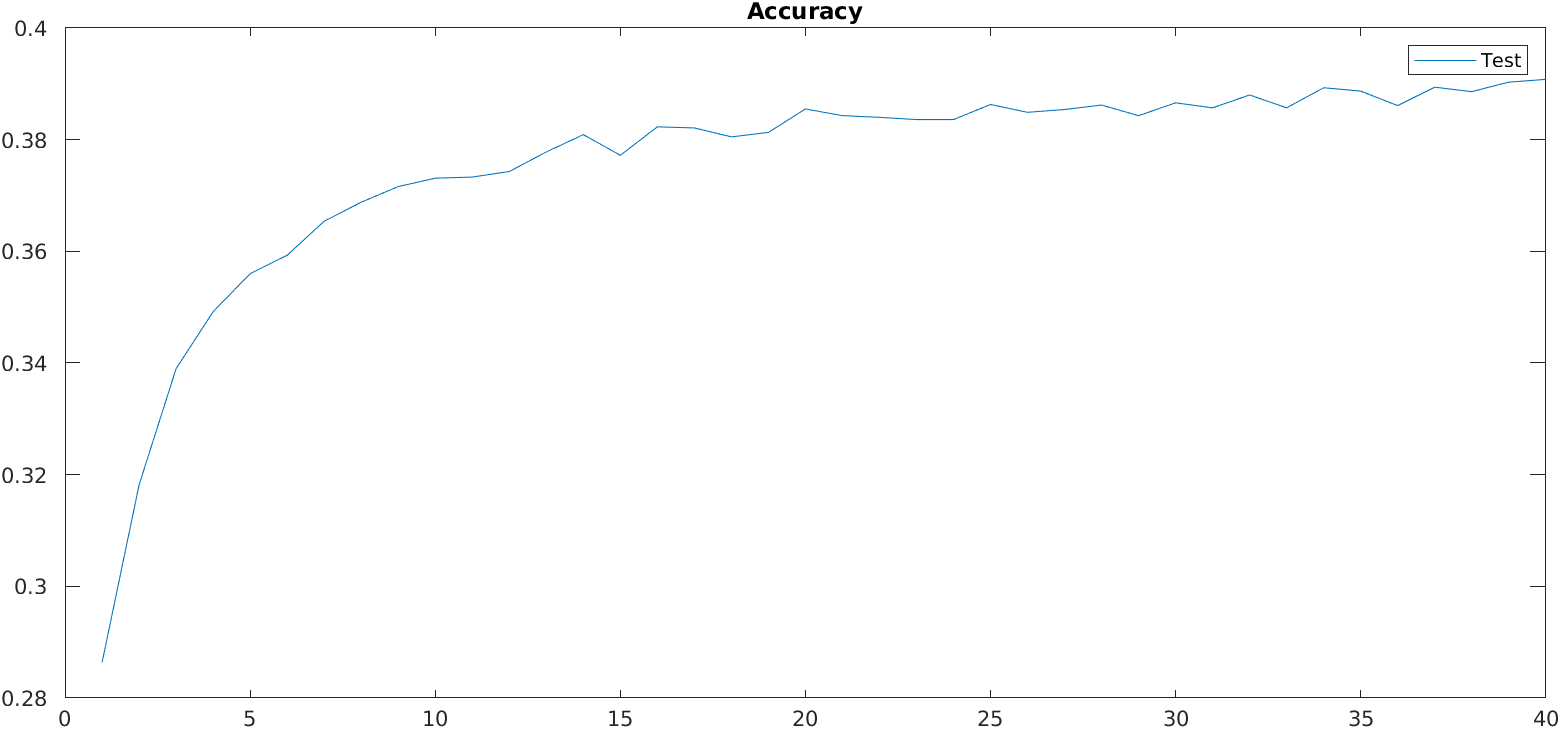
\includegraphics[width=\textwidth]{../code/result_pics/lambda=0, n_epochs=40, n_batch=100, eta=.001/accuracy.png}
        \caption{Experiment 2 Accuracy (lambda=0, n\_epochs=40, n\_batch=100, eta=0.001)}
        \label{fig:accuracy2}
    \end{figure}

    \begin{figure}[ht]
        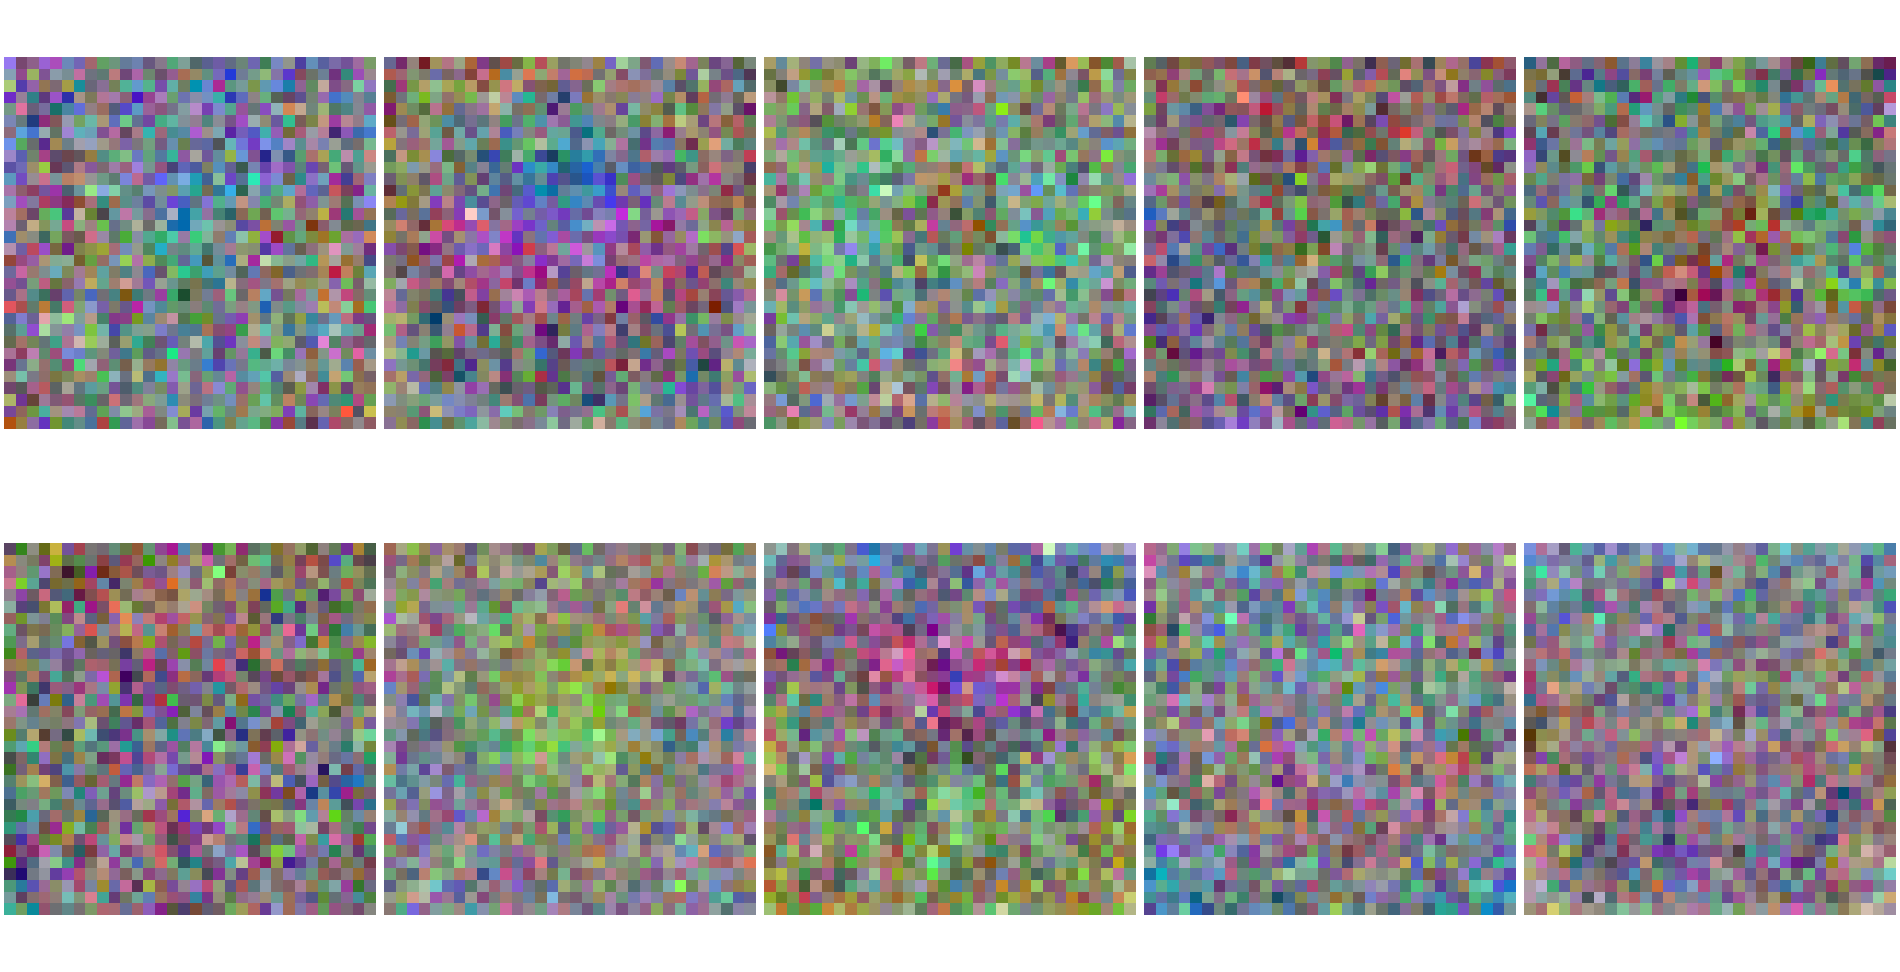
\includegraphics[width=\textwidth]{../code/result_pics/lambda=0, n_epochs=40, n_batch=100, eta=.001/weights.png}
        \caption{Experiment 2 Weights (lambda=0, n\_epochs=40, n\_batch=100, eta=0.001)}
        \label{fig:weights2}
    \end{figure}

\clearpage
\subsection{Experiment 3 diagrams}
% lambda = 0.1\\
% n\_epochs = 40\\
% n\_batch = 100\\
% eta = 0.001\\
In this experiment we use a small regularization term. This results in a smaller training loss compared to the previous run.
But we have still a big difference between training and validation which could mean that we overfit. We start to see some more distinct patterns
in the weight matrices.

    \begin{figure}[ht]
        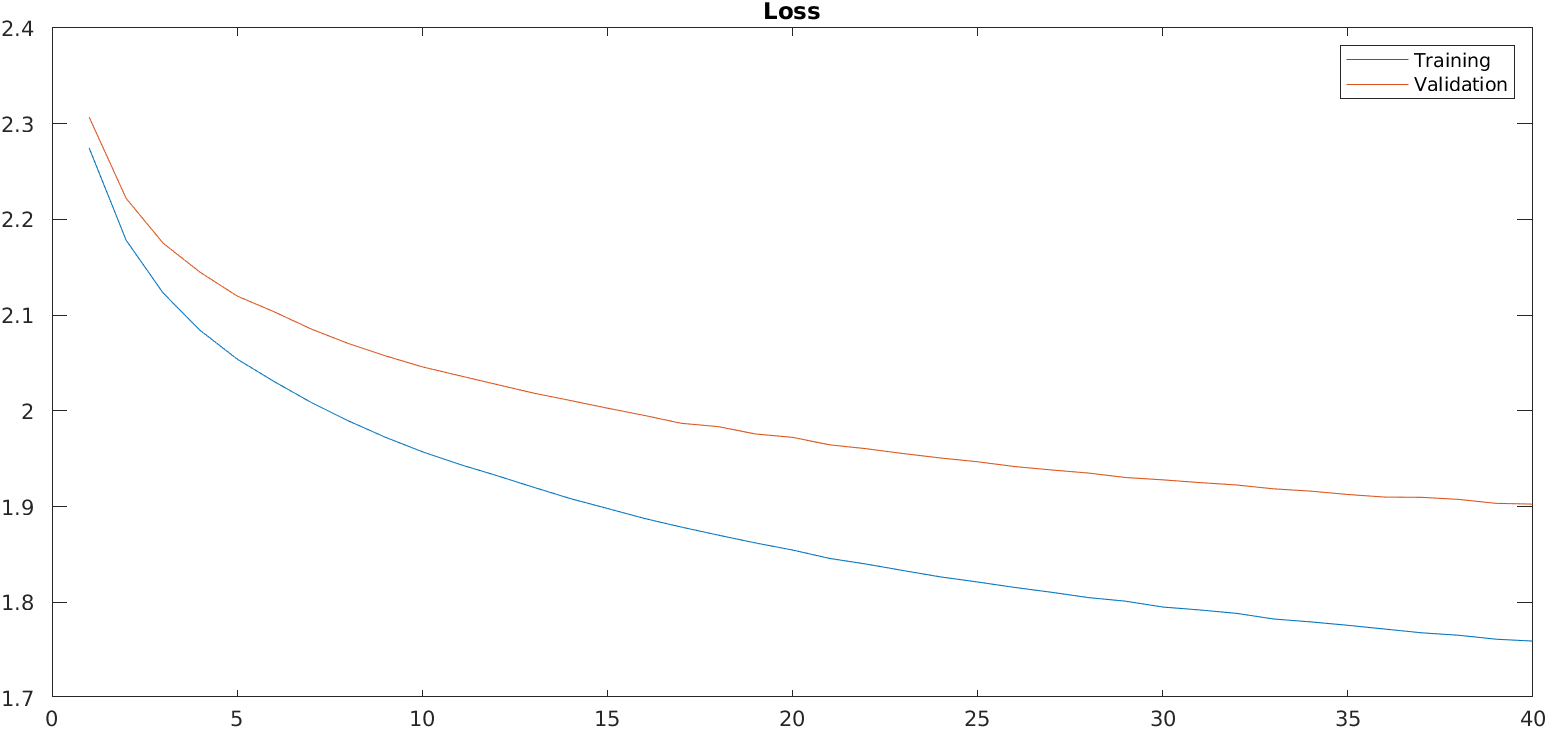
\includegraphics[width=\textwidth]{../code/result_pics/lambda=.1, n_epochs=40, n_batch=100, eta=.001/loss.png}
        \caption{Experiment 3 Loss (lambda=0.1, n\_epochs=40, n\_batch=100, eta=0.001)}
        \label{fig:loss3}
    \end{figure}

    \begin{figure}[ht]
        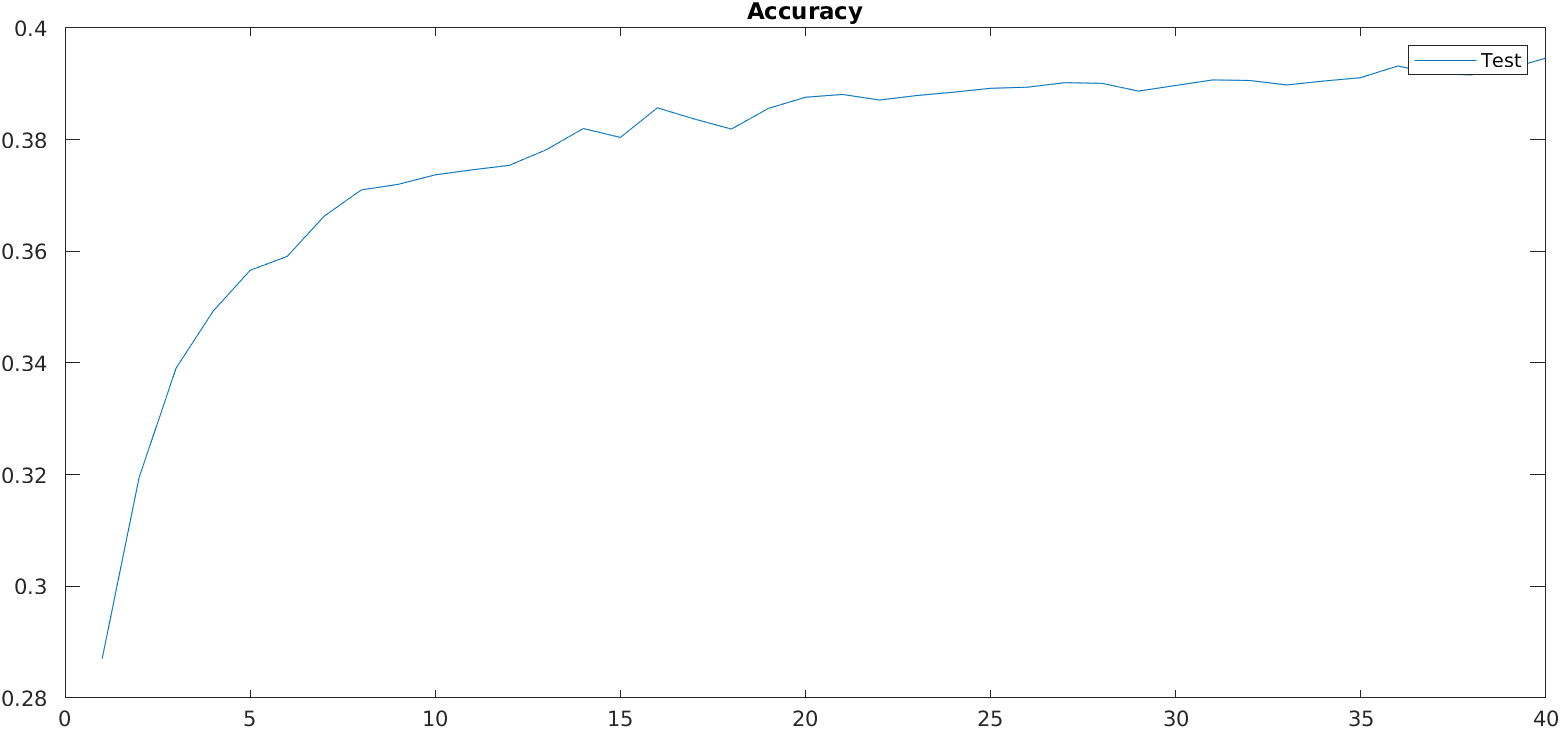
\includegraphics[width=\textwidth]{../code/result_pics/lambda=.1, n_epochs=40, n_batch=100, eta=.001/accuracy.png}
        \caption{Experiment 3 Accuracy (lambda=0.1, n\_epochs=40, n\_batch=100, eta=0.001)}
        \label{fig:accuracy3}
    \end{figure}

    \begin{figure}[ht]
        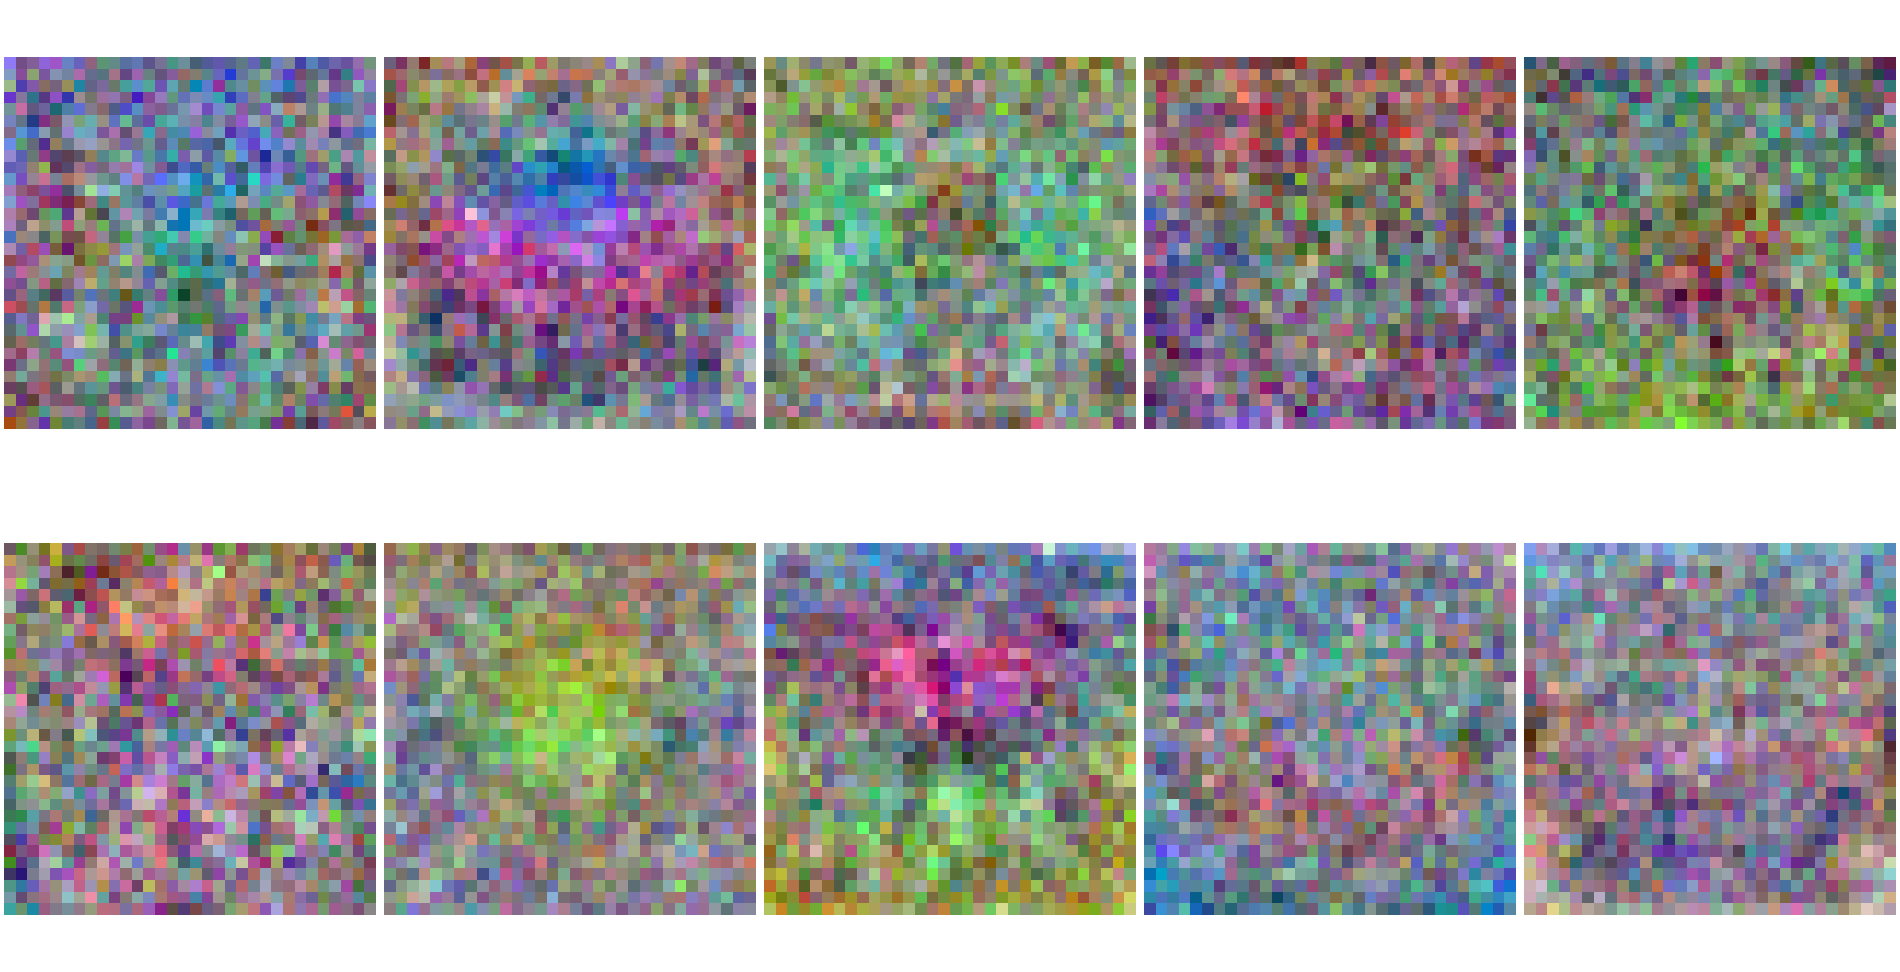
\includegraphics[width=\textwidth]{../code/result_pics/lambda=.1, n_epochs=40, n_batch=100, eta=.001/weights.png}
        \caption{Experiment 3 Weights (lambda=0.1, n\_epochs=40, n\_batch=100, eta=0.001)}
        \label{fig:weights3}
    \end{figure}

\clearpage
\subsection{Experiment 4 diagrams}
% lambda = 1\\
% n\_epochs = 40\\
% n\_batch = 100\\
% eta = 0.001\\
In this experiment we use an even bigger regularization term. That results in a slightly reduced accuracy but also the training 
and validation loss are close. That could mean that we are not overfitting anymore.\\
In the weight matrix we see that we start to learn some patterns that looks similar to the images of the corresponding classes. 
Maybe with more training these patterns become even more visible.

    \begin{figure}[ht]
        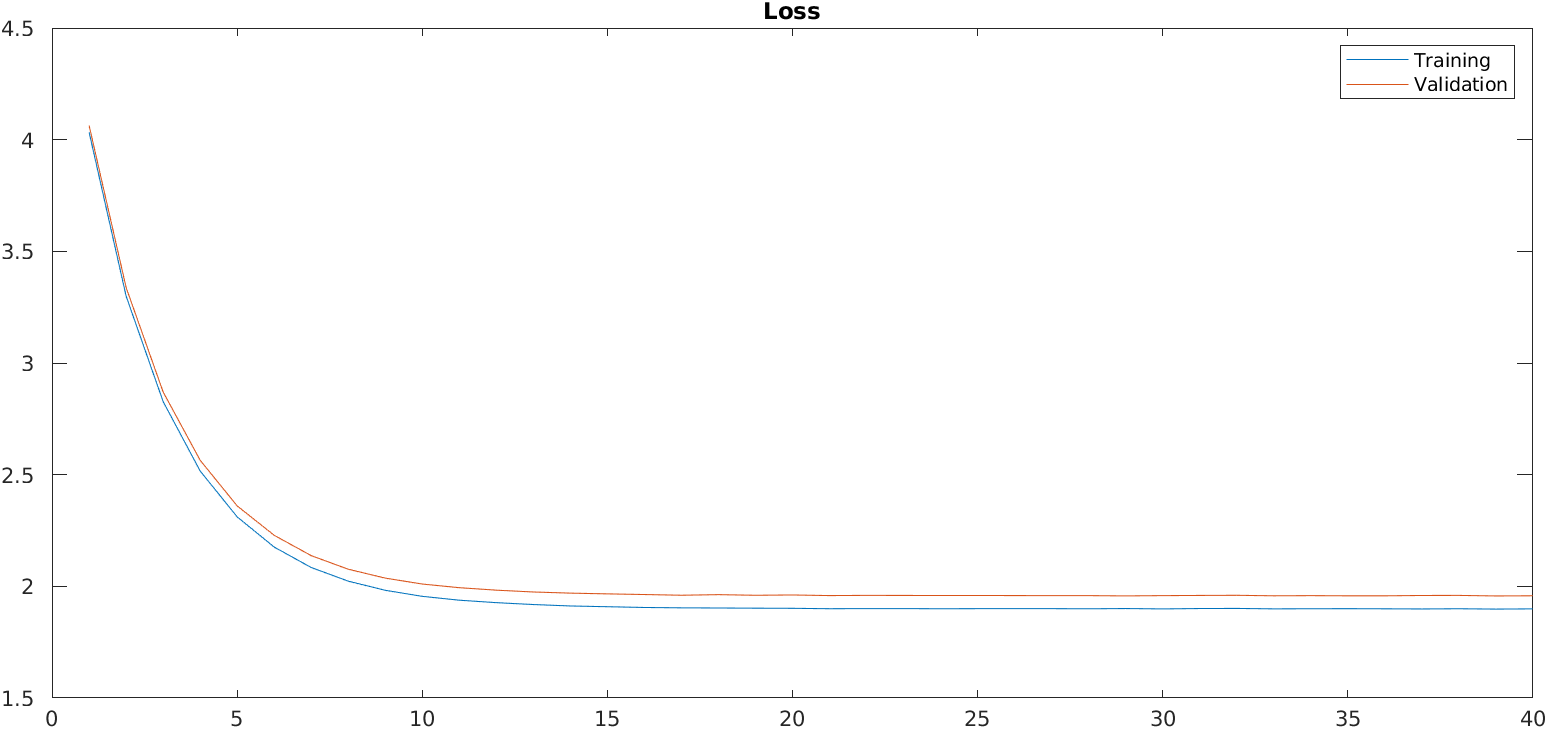
\includegraphics[width=\textwidth]{../code/result_pics/lambda=1, n_epochs=40, n_batch=100, eta=.001/loss.png}
        \caption{Experiment 4 Loss (lambda=1, n\_epochs=40, n\_batch=100, eta=0.001)}
        \label{fig:loss4}
    \end{figure}

    \begin{figure}[ht]
        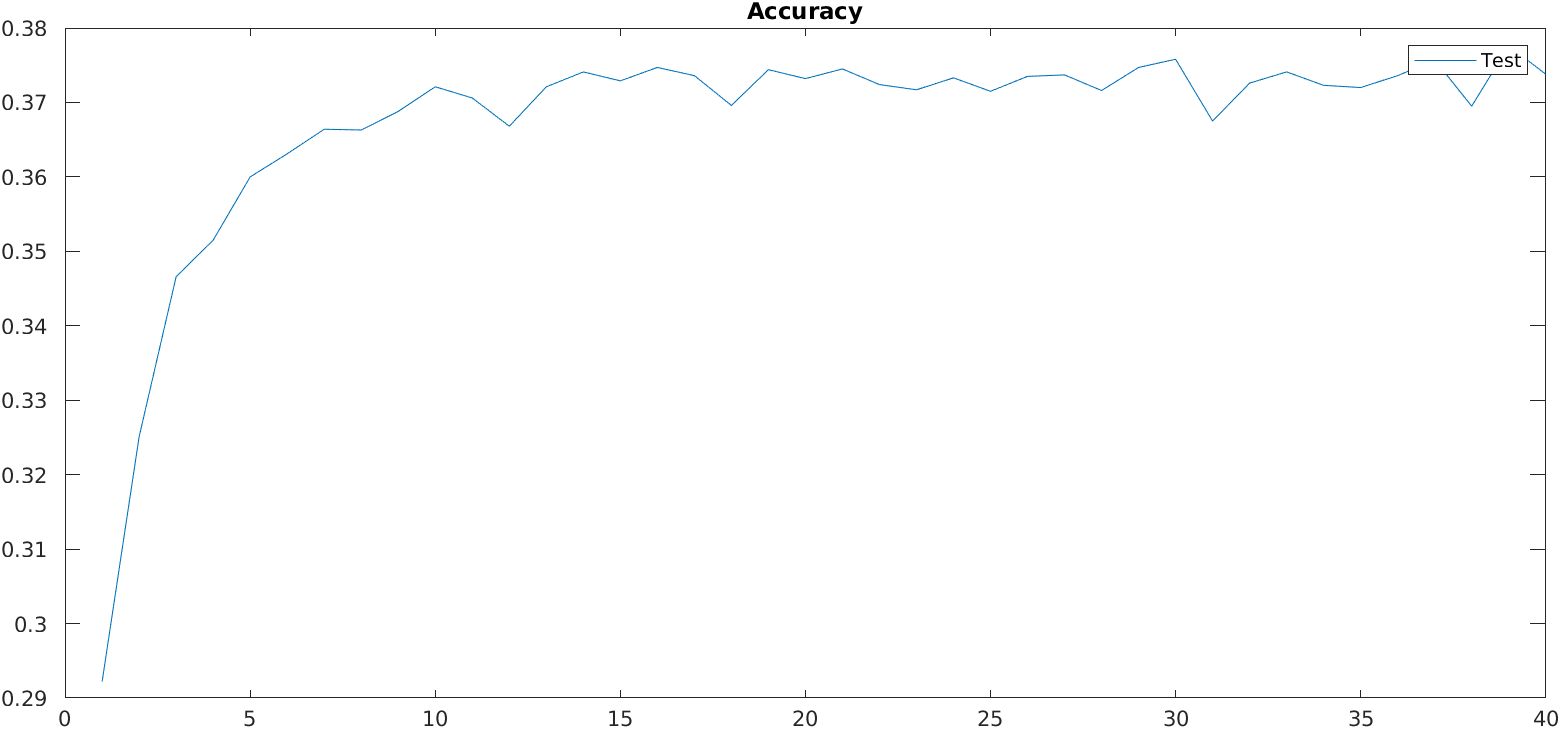
\includegraphics[width=\textwidth]{../code/result_pics/lambda=1, n_epochs=40, n_batch=100, eta=.001/accuracy.png}
        \caption{Experiment 4 Accuracy (lambda=1, n\_epochs=40, n\_batch=100, eta=0.001)}
        \label{fig:accuracy4}
    \end{figure}

    \begin{figure}[ht]
        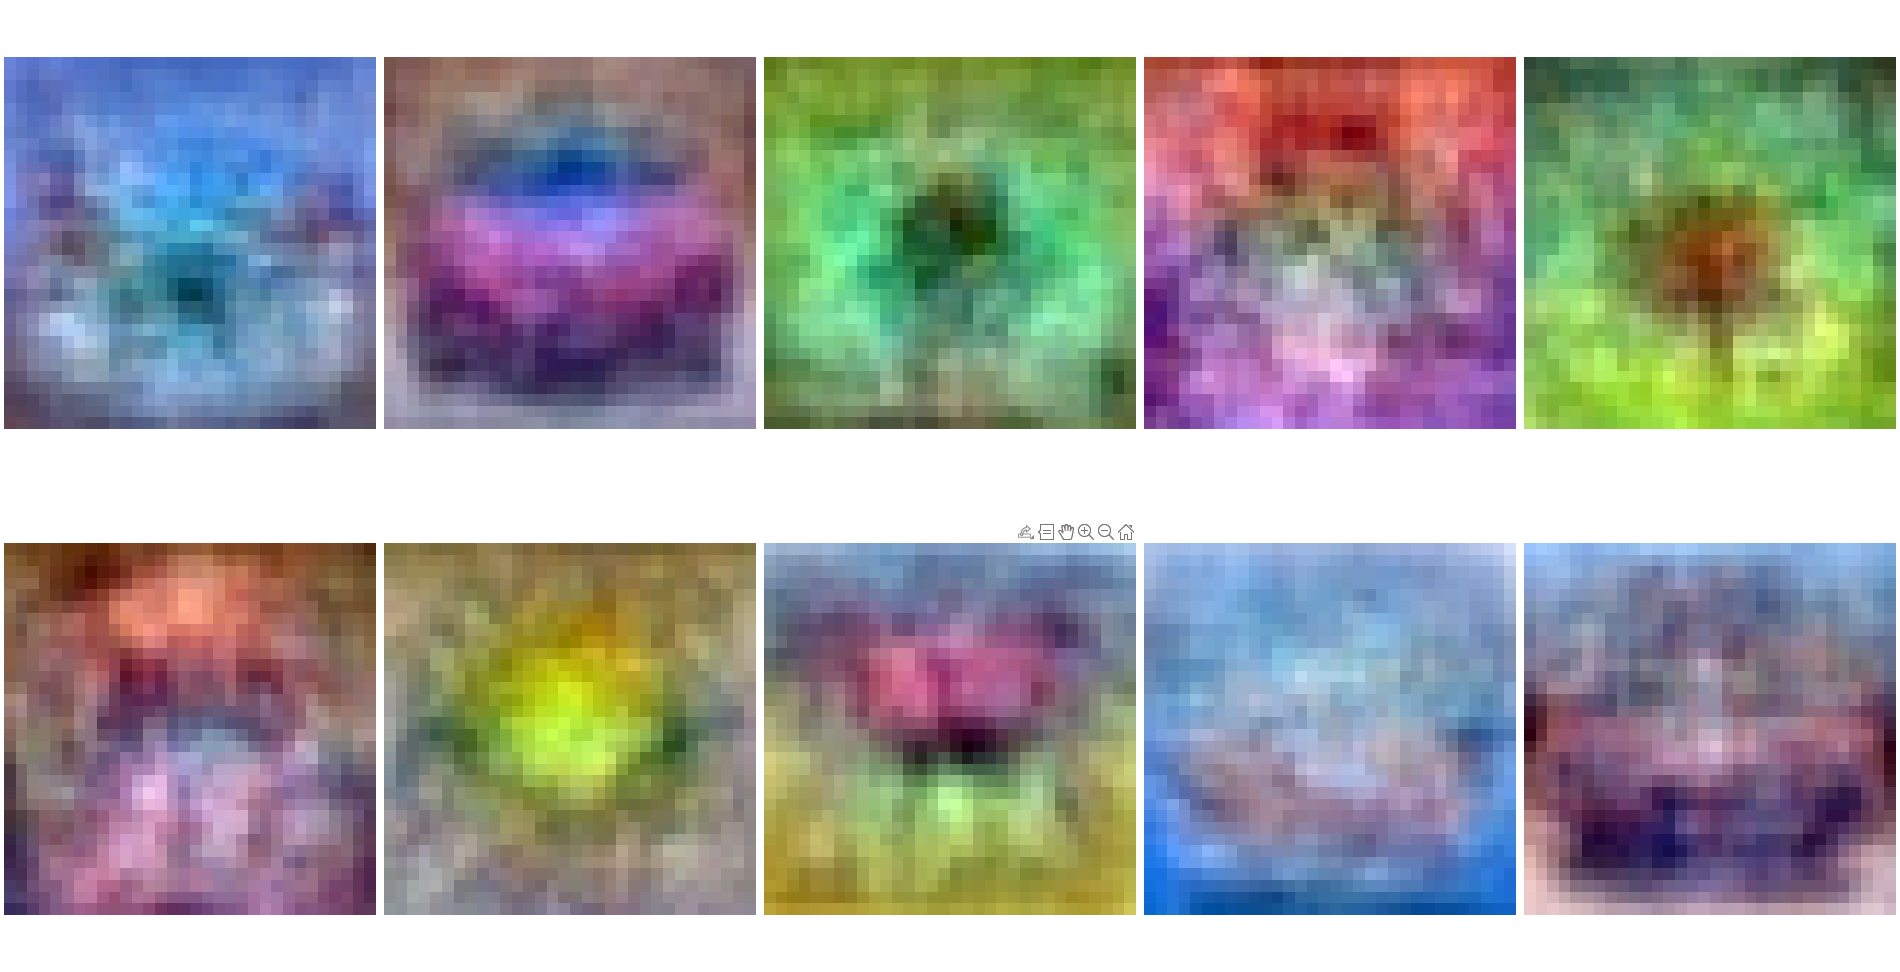
\includegraphics[width=\textwidth]{../code/result_pics/lambda=1, n_epochs=40, n_batch=100, eta=.001/weights.png}
        \caption{Experiment 4 Weights (lambda=1, n\_epochs=40, n\_batch=100, eta=0.001)}
        \label{fig:weights4}
    \end{figure}

\clearpage

\section{Conclusion}
Increasing the amount of regularization reduces the accuracy but also prevents the network from overfitting. The choice of the correct
learning rate is very important for the networks ability to learn, as we can see when comparing Experiment 1 and Experiment 2. The learning rate
has a huge impact on the accuracy.